\documentclass{article}
\usepackage[utf8]{inputenc}
\usepackage{hyperref}
\usepackage{amsmath}
\usepackage{amsfonts}
\usepackage{amssymb}
\usepackage{braket}
\usepackage{graphicx}
\usepackage{dsfont}
\usepackage{enumitem}
\usepackage{physics}

\graphicspath{ {./img/} }

\title{Introduction to Quantum Information and Computing - Notes}
\author{Aayush Acharya, Arnav Negi, Kriti Gupta, Manav Shah, Muhammed Shamil K,\\ Shiven Sinha, Shrikara A, Swayam Agrawal, Vineeth Bhat, Yash Adivarekar} % add contributors
\date{February 2023}
\begin{document}


\maketitle
\vfill
\tableofcontents
\newpage
\pagenumbering{arabic}


%2023-01-31

\section{Introduction}
\begin{itemize}
	\item Quantum computing - "Natural generalization of computing".
\end{itemize}
\begin{itemize}
	\item Quantum computers are computers that obey quantum physics.
\end{itemize}


\subsection{Why quantum computing?}
\begin{itemize}
	\item Extended Church Turing Thesis (ECT): Any algorithmic process can be efficiently simulated by a probabilistic Turing machine.
\end{itemize}
\begin{itemize}
	\item David Deutsch:-Is there a physical model of computation that violates ECT?
\end{itemize}
\begin{itemize}
	\item Computation devices built using the principles of quantum physics can offer a stronger version to their thesis.
\end{itemize}\begin{itemize}
	\item Do quantum computers that obey quantum mechanics violate ECT?
\end{itemize}\begin{itemize}
	\item Feynman asks if we can simulate quantum physics on a classical computer.
\end{itemize}\begin{itemize}
	\item Number of variables to keep track of is exponential in the size of the quantum system. For example, for a 100 electron system,${2^{100}}$ bits are needed in comparison to 100 qubits.
\end{itemize}

\section{Quantum computing in the circuit model\\ (Postulates of Quantum mechanics in action)}
\subsection{State Preparation}
\begin{itemize}
	\item Prepare the quantum computer in a given initial state\\
	      ${|\psi_{0}}\rangle$=${|0\rangle^{\otimes n}}$
\end{itemize}\begin{itemize}
	\item ${|0\rangle}$=${\begin{pmatrix}
					      1 \\
					      0
				      \end{pmatrix}}$\\
	      ${|0\rangle\otimes|0\rangle}$=${|0\rangle^{\otimes2}}$=${|0\rangle|0\rangle}$=${|00\rangle}$
\end{itemize}

\subsection{Evolution}
\begin{itemize}
	\item Schrodinger's equation :\\\\
	      ${i\frac{d|\psi\rangle}{dt}}$=${H|\psi\rangle}$\\\\
	      ${|\psi(t)\rangle}$=${e^{-iHt}}|\psi(0)\rangle$
\end{itemize}
\begin{itemize}
	\item H: Hamiltonian observable for energy
\end{itemize}
\begin{itemize}
	\item ${u_t} = {e^{-iHt}}$
\end{itemize}
\begin{itemize}
	\item The initial state ${|\psi_0\rangle}$ evolves based on a series of unitary operators  \\
	      ${|\psi_f\rangle}$=${u_tu_{t-1}u_{t-2}...u_2u_1|\psi_0\rangle}$\\
	      where each ${u_i}$ is a quantum gate
\end{itemize}

\subsection{Measurement}

\begin{itemize}
	\item Measure the final state in the computational basis: M={${|j\rangle\langle j|}$ where ${j\in \{0,1\}^n}$}
\end{itemize}
\begin{itemize}
	\item Observe ${|f\rangle}$ with probability p such that: \\
	      ${p=|\langle f|\psi_f\rangle|^2}$
\end{itemize}

%2023-02-07

\section{Classical Logic Gates}

Any boolean function $f:\{0,1\}^n \xrightarrow{} \{0,1\} $ can be written as a propositional formula of $n$ variables.
A universal gate is a gate which can implement any Boolean function $f$ without need to use any other gate type.

\subsection{Reversibility of Logic Gates}

Logical reversibility means that the output can be computed from the input, and vice versa. Reversible functions are bijective. This means that reversible gates (and circuits, i.e. compositions of multiple gates) have the same number of inputs as outputs.

A NOT gate is logically reversible because it can be undone.

The exclusive or XOR gate is irreversible because its two inputs cannot be unambiguously reconstructed from its single output, or alternatively, because information erasure is not reversible.

A motivation for implementing reversible computing is that they offer to improve the computational energy efficiency of computers.

\section{Shannon Entropy}

Shannon entropy is a measure of the amount of uncertainty or information contained in a quantum state. It is defined as:
$\ \sum_{i} -p_i \log(p_i)$

Example:
Consider a qubit with initial probability distrubution $P:\{0.5,0.5\}$.We reset this qubit and we are asked to calculate the change in entropy.

The initial entropy = $\ -0.5*log(0.5) - 0.5*log(0.5)$\ = $\log(2)$.

The final entropy is 0 as the qubit is reset and thus no probabilistic measure.

Hence $\Delta S = -log(2)$

\section{Landauer's Principle}

Landauer's principle is a fundamental principle in quantum information theory that relates the amount of irreversible information loss in a computation to the physical process of erasing information. In essence, the principle states that erasing information must necessarily generate entropy, and that the minimum amount of energy required to perform an erasure is proportional to the entropy generated.

It can be formally stated as : Any irreversible operation that erases one bit of information must necessarily generate at least $k_B ln 2$ units of entropy, where $k_B$ is the Boltzmann constant. This means that the minimum energy required to perform an erasure is given by:

$E = k_B T \ln 2$ where $T$ is the temperature of the system in which the erasure is performed.

\section{Clausius Inequality}

The Clausius inequality is a fundamental principle of thermodynamics that places a limit on the amount of work that can be extracted from a system during a thermodynamic process.Mathematically: \\\\
$\Delta Q \geq k_B T \Delta S$ \\\\
Here $\Delta S$ is the decrease in entropy of the system or increase in entropy of environment. $\Delta Q$ denotes the heat lost by the system to the environment.

\section{Demonstrating the relationship between Measurement, Information and Thermodynamics}

The Szilard Engine and Maxwell's Demon are two thought experiments in quantum mechanics that highlight the role of information and measurement in thermodynamics.
\subsection{Szilard Engine}
The Szilard Engine consists of a single particle confined in a box with a partition in the middle. The box is initially in a state of thermal equilibrium with its environment. The partition is moved to one side of the box, and the position of the particle is measured. If the particle is found on one side of the box, then the partition is locked into place, creating a smaller box on that side. This process can be repeated until the particle is confined to a small box, and the work that can be extracted from the process can be used to do useful work. \\\\\
This engine thus demonstrates that measurement and information are intimately connected to thermodynamics. In particular, the act of measuring the position of the particle changes the state of the system, and this change can be used to extract work from the system. This suggests that information is a form of physical resource that can be converted into work.

\section{Reversible Logic Gates}

\subsection{Fredkin Gate}
Also know as Controlled SWAP Gate

The Fredkin gate has three input bits and three output bits, which we refer to
as a, b, c and a', b', c', respectively. The bit c is a control bit, whose value is not changed by the action of the Fredkin gate, that is, c' = c. The reason c is called the control bit is because it controls what happens to the other two bits, a and b. If c is set to 0 then a and b are left alone, a' = a, b' = b. If c is set to 1, a and b are swapped, a' = b, b' = a. It is easy to see that the Fredkin gate is reversible, because given the output a', b, c', we can determine the inputs a, b, c. In fact, to recover the original inputs a, b and c we need only apply another Fredkin gate to a', b', c

\begin{figure}[htp]
	\centering
	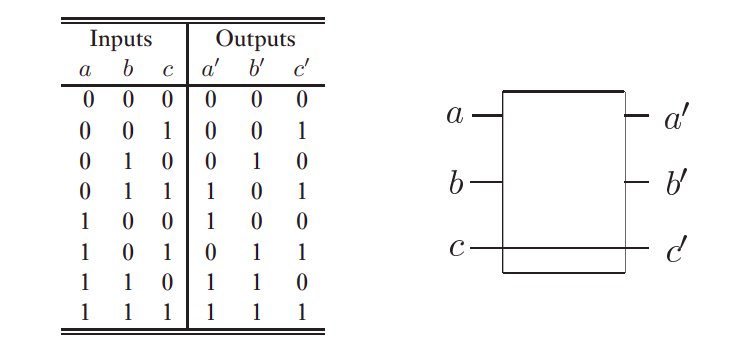
\includegraphics[width=10cm]{fredkin.png}
\end{figure}

The Fredkin gate is not only reversible, it’s a universal logic gate
as well.\\

Reversible AND Gate (R-AND):
\begin{figure}[htp]
	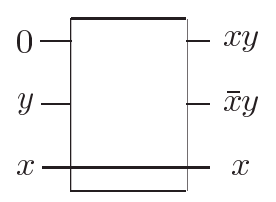
\includegraphics[width=5cm]{rand.png}
\end{figure}
\\

Reversible OR Gate (R-OR):
\begin{figure}[htp]
	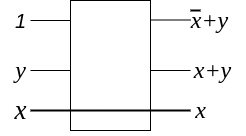
\includegraphics[width=5cm]{ror.png}
\end{figure}
\\

Reversible NOT Gate (R-NOT):
\begin{figure}[htp]
	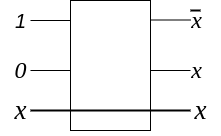
\includegraphics[width=5cm]{rnot.png}
\end{figure}

\subsection{CNOT Gate}
Controlled-NOT Gate: This gate has two input qubits, known as the control qubit and the target qubit.The action of the gate may be described as follows. If the control qubit is set to 0, then the target qubit is left alone. If the control qubit is set to 1, then the target qubit is flipped. The following image shows the circuit and the unitary matrix corresponding to the gate.

\begin{figure}[htp]
	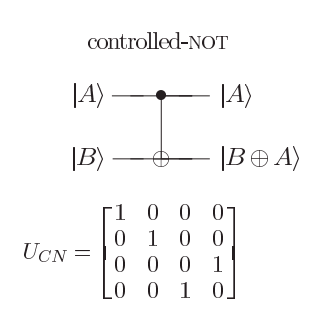
\includegraphics[width=5cm]{cnot.png}
\end{figure}

The reason the CNOT gate is not universal on its own is because it can only generate entangled states where the control and target qubits are either both 0 or both 1. This limits the set of transformations that can be generated.Reversibility is implied from the truth table.

%2023-02-10
\section{Tofolli Gate}

Also known as $CCNOT$ Gate.

\begin{figure}[htp]
    \centering
    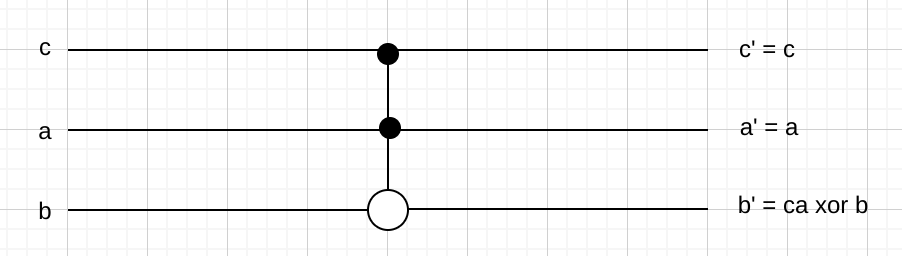
\includegraphics[width=10cm]{tofolli.png}
\end{figure}

The $CCNOT$ gate preserves the control, $c$, and first input, $a$, and only performs an operation on the last input, $b$, to give the output $$b'=ca \oplus b$$

which means that for $b$ to be flipped, both $a$ and $c$ must be 1.

Further, this gate is universal and reversible.

\section{Some problems}

\begin{enumerate}
    \item We receive some garbage bits that we don't require in the output of a quantum gate. For example, consider the operation carried out by a unitary $u_f$:
    $$|x,0,0\rangle \xrightarrow[]{u_f} \Sigma_y \alpha |y\rangle |f(y)\rangle |g(y)\rangle $$
    The term $|g(y)\rangle$ might not be needed and is termed as garbage or ancillary.
    \item The garbage bits are entangled with the input and cannot be reset as it will make the operation irreversible.
    \item We cannot measure the garbage register either as measurement will collapse the superposition to a particular state which isn't desirable.
\end{enumerate}
This is solved using uncomputation.

\section {Uncomputation}

Say we wish to obtain the solution $|f(x)\oplus y \rangle$ given the inputs $|x\rangle$ and $|y\rangle$ as follows:

$$|x\rangle |0\rangle |0\rangle |y\rangle \xrightarrow[]{u_f} |x\rangle |f(x)\rangle |g(x)\rangle |y\rangle$$

Where the unitary $u_f$ is applied on the first three qubits.

$$|x\rangle |f(x)\rangle |g(x)\rangle |y\rangle \xrightarrow[]{CNOT_{2,4}} |x\rangle |f(x)\rangle |g(x)\rangle |f(x) \oplus y\rangle$$

We then use the $CNOT$ gate on the 2nd and 4th qubits, i.e., $|f(x)\rangle$ and $|y\rangle$

$$|x\rangle |f(x)\rangle |g(x)\rangle |f(x) \oplus y\rangle \xrightarrow[]{u^{-1}_f} |x\rangle |0\rangle |0\rangle |f(x) \oplus y\rangle$$

We use the inverse of the unitary operation used earlier to uncompute the 2nd and 3rd bits.

All of these operations are represented by the short hand notation:

\begin{figure}[htp]
    \centering
    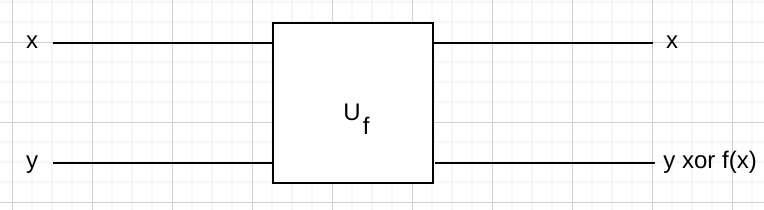
\includegraphics[width=10cm]{uncomputation.png}
\end{figure}

\section {Quantum Circuits}

We note that
\begin{enumerate}
    \item Quantum gates are unitary operations on quantum states.
    \item There exists a set of universal gates for quantum circuits usually denoted by $G_O$, which contains a small number of single as well as two qubit gates.
\end{enumerate}

\subsection{Single Qubit Gates}

These include 

\begin{enumerate}
    \item Pauli matrices (which have been elucidated on earlier in the first half)
    \item Hadamard matrix

    $$H = \frac{1}{\sqrt{2}} \begin{bmatrix}
            1 & 1\\
            1 & -1
    \end{bmatrix}$$

    They transform from the basis $\{|0\rangle, |1\rangle\}$ to $\{|+\rangle, |-\rangle\}$.

    $$H|0\rangle = |+\rangle = \frac{1}{\sqrt{2}}(|0\rangle + |1\rangle)$$    
    $$H|1\rangle = |-\rangle = \frac{1}{\sqrt{2}}(|0\rangle - |1\rangle)$$    
    
    \item Phase change matrices

    $$R_{\phi} = \begin{bmatrix}
            1 & 0\\
            0 & e^{i\phi}    
    \end{bmatrix}$$

    The phase change matrix adds a change of phase $\phi$ to the the state $|1\rangle$ as $$R_{\phi}(|\alpha |0\rangle + \beta |1\rangle) = |\alpha |0\rangle + e^{i\phi}\beta |1\rangle$$

    Some accepted ways of denoting common phase changes are $S=R_{\frac{\pi}{2}}$ and $T=R_{\frac{\pi}{4}}$.
    
\end{enumerate}

\subsection{Two Qubit Gates}

\subsubsection{Controlled two qubit gates}

For example, if we wish to apply the unitary $u$ only on the second state in $|ab\rangle$, i.e., as a $controlled$ operation on a single qubit gate, we use the circuit:

\begin{figure}[htp]
    \centering
    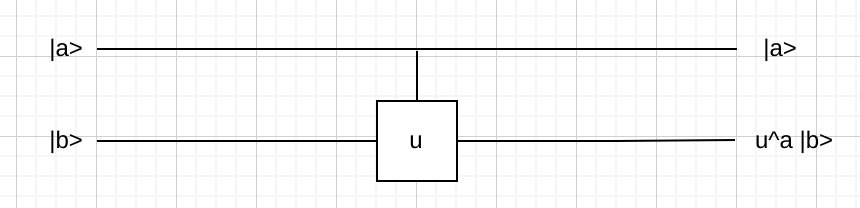
\includegraphics[width=10cm]{twoqubit.png}
\end{figure}

The matrix representation of the operation is

$$
    U = \begin{bmatrix}
        \begin{matrix}
            1 && 0\\
            0 && 1
        \end{matrix}
        && 
        \begin{matrix}
            0 && 0\\
            0 && 0
        \end{matrix}
        \\
        \begin{matrix}
            0 && 0\\
            0 && 0
        \end{matrix}
        && 
        u
    \end{bmatrix}
$$

The operations carried out are:
$$|00\rangle \xrightarrow[]{U} |00\rangle$$
$$|01\rangle \xrightarrow[]{U} |01\rangle$$
$$|10\rangle \xrightarrow[]{U} |1\rangle(u|0\rangle)$$
$$|11\rangle \xrightarrow[]{U} |1\rangle(u|1\rangle)$$

For example, if we wish to model the $CNOT$ gate, we take $u=\sigma _x$ if the above circuit.

\subsubsection{Another example of two qubit gates}

Consider the following circuit

\begin{figure}[htp]
    \centering
    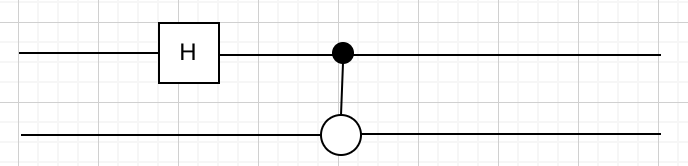
\includegraphics[width=10cm]{extwoqubit.png}
\end{figure}

If we apply this circuit on the input $|00\rangle$, then we can model the output using the following calculations

$$|00\rangle \xrightarrow[]{H \otimes \mathbf{I}} |+0\rangle = \frac{1}{\sqrt{2}}(|00\rangle + |10\rangle)$$

$$\frac{1}{\sqrt{2}}(|00\rangle + |10\rangle) \xrightarrow[]{CNOT} \frac{1}{\sqrt{2}}(|00\rangle + |11\rangle)$$
%2023-02-14

\section{General Quantum Circuits}
Elementary gates can be composed into bigger quantum circuits.

This can be done in two ways:
\begin{enumerate}
    \item Tensor product
    \item Ordinary matrix product
\end{enumerate}

\subsection{Tensor Product}
Combination of gates applied to different registers.

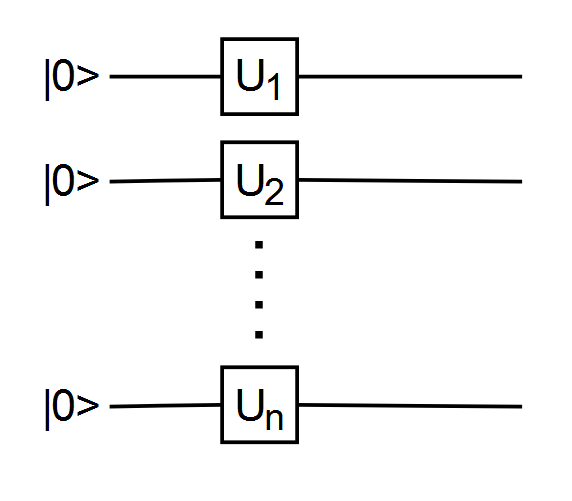
\includegraphics[scale=0.5]{q1.png}

\begin{center}
$    U_{1} \ket{0} \otimes U_{2} \ket{0} ... U_{n} \ket{0}
    = (U_{1} \otimes U_{2} ... \otimes U_{n}) \ket{0...0}$


    $= U^{\otimes n} \ket{0^{n}}$ when $U_{i}=U \forall i$
    
\end{center}

$(U_{1} \otimes U_{2} ... \otimes U_{n}) $ is a $2^{n}$ dimension unitary.

\subsection{Ordinary Matrix Product}
Combination of gates applied to same register.

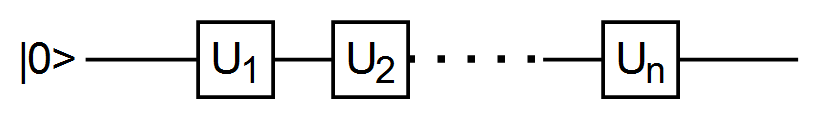
\includegraphics[scale=0.5]{q2.png}

Output, $\ket{\psi} = (U_{n}...U_{1})\ket{0}$

Here, for all $U$, dim = $2 \times 2 $ (if all $U_{i}s$ are single qubit)

\section{Cost of Quantum Circuits}

\begin{enumerate}
    \item Gate complexity
    \item Depth complexity 
    \item Query complexity
\end{enumerate}
\subsection{Query Complexity}
Query complexity is decided by number of queries made to a blackbox, $U_{f}$.

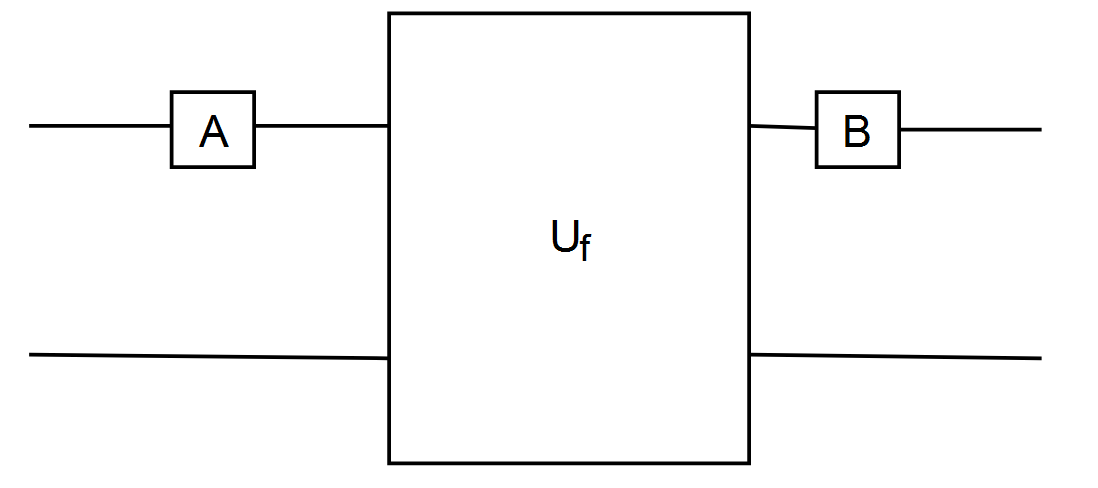
\includegraphics[scale=0.3]{q3.png}

Gates added before and after the blackbox to prepare desired input/output state do not affect the complexity. 

\section{State produced by Hadamard Gate}

\subsection{Single Hadamard gate}

\begin{gather*}
    H = \frac{1}{\sqrt{2}} 
    \begin{pmatrix}
    1 & 1\\
    1 & -1
    \end{pmatrix}
\end{gather*}
\begin{gather*}
    H \ket{0} = \frac{1}{\sqrt{2}} (\ket{0}+\ket{1})
\end{gather*}
\begin{gather*}
    H \ket{1} = \frac{1}{\sqrt{2}} (\ket{0}-\ket{1})
\end{gather*}

when $x \in \{0, 1\}$,

\begin{gather*}
    H \ket{x} = \frac{1}{\sqrt{2}} (\ket{0}+ (-1)^{x}\ket{1})
    =  \frac{1}{\sqrt{2}} \sum \limits _{z \in \{0,1\}} (-1)^{xz} \ket{z}
\end{gather*}

\subsection{N Hadamard gates}
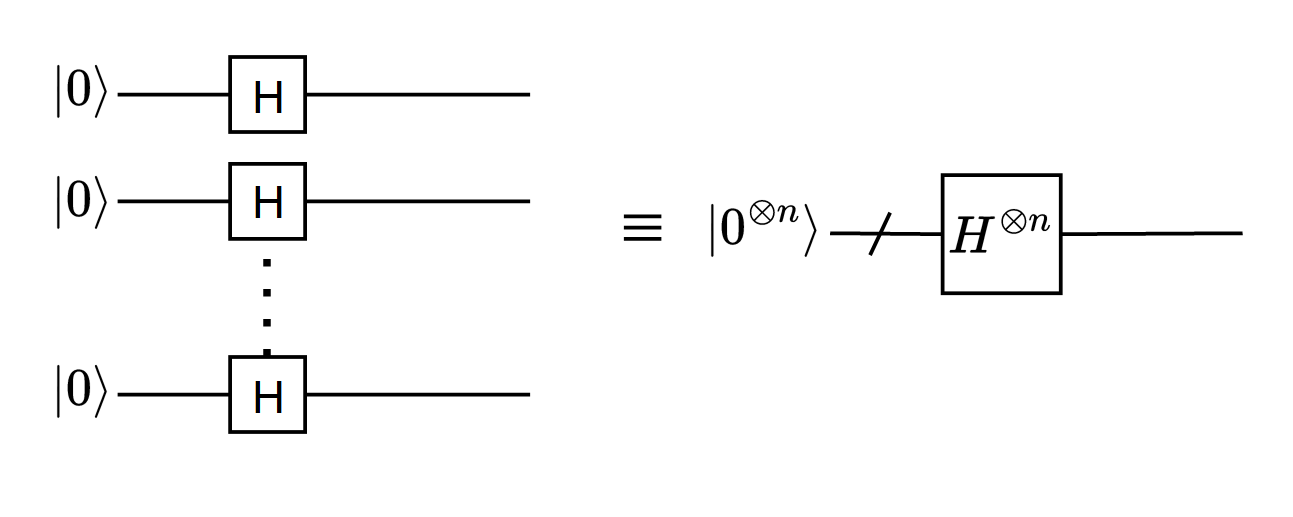
\includegraphics[scale=0.3]{q4.png}
$H^{\otimes n} = H \otimes H ... \otimes H$

\begin{align*}
Output &= \ket{+^{\otimes n}}\\
&= \frac{1}{\sqrt{2}^{n}} (\ket{0} + \ket{1}) \otimes \frac{1}{\sqrt{2}} (\ket{0} + \ket{1}) ... \otimes \frac{1}{\sqrt{2}} (\ket{0} + \ket{1}) \\
&= \frac{1}{\sqrt{2}^{n}} (\ket{0...000} + \ket{0...001} + \ket{0...010} ...)\\
&= \frac{1}{\sqrt{2}^{n}} \sum (\text{basis of n qubits)}\\\\
H^{\otimes n} \ket{0^{\otimes n}} &= \frac{1}{\sqrt{2}^{n}} \sum \limits _{z \in {0,1}^{n}} \otimes \ket{z}\\\\
H^{\otimes n} \ket{x} &= \frac{1}{\sqrt{2}^{n}} \sum \limits _{z \in {0,1}^{n}} \otimes (-1)^{x \cdot z}\ket{z}
\end{align*}

\section{Universality of Quantum Gates}
Can any U be decomposed into a combination of unitaries/gates from some finite set?

\begin{enumerate}
    \item {CNOT, all single qubit gates} $\equiv$ universal set for QC $\xrightarrow{}$ but, not finite
    \item{CNOT, H, T} = G \} Good approximation for any quantum gate.
\end{enumerate}

\subsection{Solovay-Kitaev Theorem}
\begin{itemize}
    \item Uses G, and each of the gates' inverse
\end{itemize}

\subsubsection{1-2 Qubit}
It is possible to approximate any unitary (gate) in one or two qubits upto an error $\epsilon$ by using only $O(polylog(\frac{1}{\epsilon})$ gates from G.

$\norm{U \ket{\psi} - U_{m} U_{m-1} ... U_{1} \ket{\psi}} \leq \epsilon$

Where $U$ is the matrix being approximated and each $U_{i} \in G$ and $m \in {polylog(\frac{1}{\epsilon})}$

\subsubsection{t-Gate}
Any '$t$' gate quantum circuit can be $\epsilon$-approximated by only $O(t \cdot polylog(\frac{1}{\epsilon})$ gates from G

\section{Quantum Parallelism}
\begin{itemize}
    \item Quantum circuits can be applied to multiple/all states in one query.
    \item But, output would still be of no use until we apply appropriate transformations to separate the outputs.
\end{itemize} 

E.g., Consider a classical circuit that computes 
\begin{align*}
    f: \{0, 1\}^{n} \rightarrow \{0, 1\}
\end{align*}
We need to run this $2^{n}$ times (once for each input) to find output for each input.
\medskip
Converting it to a quantum circuit but replacing gates with reversible unitaries,
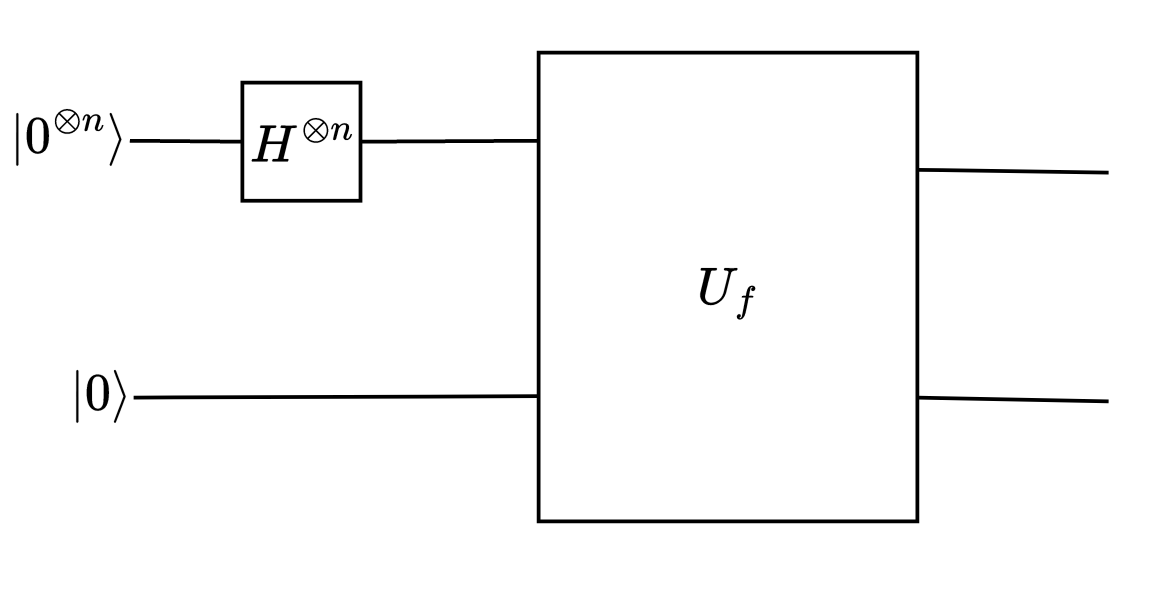
\includegraphics[scale=0.5]{q5.png}
$Output, \ket{\psi} = \frac{1}{\sqrt{2}^{n}} \sum \limits _{z \in \{0, 1\}^{n}} \ket{z} \ket{f(\ket{z})} $

%2023-02-17

\section{Phase Kickback Oracle}
Consider the CNOT gate where $U_f$ denotes the unitary operation CNOT.\\
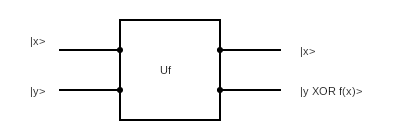
\includegraphics{CNOT.png}
The action of $U_f$ is given by:
\begin{align*}
	|x\rangle|y\rangle \xrightarrow{U_f} & |x\rangle|y\rangle \text{ if }f(x)=0            \\
	                                     & |x\rangle|\overline{y}\rangle \text{ if }f(x)=1 \\
\end{align*}
$|x\rangle,|y\rangle \in \{0,1\}$
\\
\\
Consider the case when $|y\rangle=|-\rangle$
\begin{align*}
	|x\rangle|-\rangle \xrightarrow{U_f} & U_f\frac{(|x\rangle|0\rangle+|x\rangle|1\rangle)}{\sqrt{2}}              \\
	=                                    & \frac{|x\rangle(|0 \oplus f(x)\rangle +|1 \oplus f(x)\rangle)}{\sqrt{2}} \\
	=                                    & |x\rangle|-\rangle \text{ if } f(x)=0                                    \\
	                                     & -|x\rangle|-\rangle \text{ if } f(x)=1                                   \\
	=                                    & (-1)^{f(x)}|x\rangle|-\rangle
\end{align*}
\\
\\
If $x \in \{0, 1\}^n$ and before $U_f$, $H^{\otimes n}$ is applied on $|x\rangle$, then the output is:
\begin{align*}
	 & U_f \frac{1}{\sqrt{2^n}}\sum_{z \in \{0,1\}^n} |z\rangle|-\rangle           &  & \textit{from the action of H}     \\
	 & =\frac{1}{\sqrt{2^n}}\sum_{z \in \{0,1\}^n} (-1)^{f(x)} |z\rangle |-\rangle &  & \textit{from the action of $U_f$}
\end{align*}

Usually, the $|-\rangle$ in the second register is dropped when writing the phase kickback since it remains unchanged in output and is considered implicit when using the phase kickback oracle.

\section{Deutsch Algorithm}
\subsection{The Problem}
Suppose $U_f$ is given as a black box for a boolean function $f: \{0,1\} \rightarrow \{0,1\}$, with the promise that either:
\begin{enumerate}[label=(\roman*)]
	\item $f(0)=f(1)$
	\item $f(0) \neq f(1)$
\end{enumerate}
How many queries do we need to make to $U_f$ to determine which of the two is true?
\subsection{Classical Reversible Computation}
Classically, two queries to $U_f$ are needed, one to determine the value of $f(0)$ and one to determine the value of $f(1)$. \\
We can then compare the two and decide which promise is true.
%%! put images here
% \\\\images of classical circuit\\
\\ 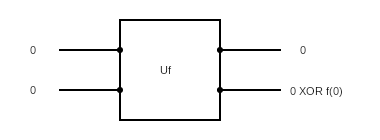
\includegraphics{classicalD0.png}
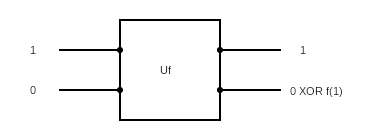
\includegraphics{classicalD1.png}

\subsection{Quantum Computation}
Consider the following quantum circuit:\\
%%! put image here
% \\\\image of quantum circuit\\\\\\
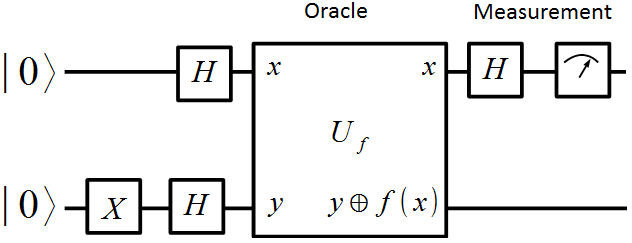
\includegraphics[scale=0.5]{The-Deutsch-Algorithm.jpg}

\subsubsection{Finding Final State}
Finding the output: \\
\begin{align*}
	|0\rangle|-\rangle \xrightarrow{H \otimes \mathbb{I}} & |+\rangle|-\rangle                                                                                                                                  &  & \text{Apply H to first register} \\
	\xrightarrow{U_f}                                     & \frac{1}{\sqrt{2}} ((-1)^{f(0)}|0\rangle + (-1)^{f(1)}|-\rangle) |-\rangle                                                                          &  & \text{Apply phase kickback}      \\
	\xrightarrow{H \otimes \mathbb{I}}                    & \frac{1}{\sqrt{2}} ((-1)^{f(0)}|+\rangle + (-1)^{f(1)}|-\rangle) |-\rangle                                                                          &  & \text{Apply H to first register} \\
	=                                                     & \frac{1}{\sqrt{2}} \left( \frac{(-1^{f(0)})(|0\rangle + |1\rangle)}{\sqrt{2}} + \frac{(-1^{f(1)})(|0\rangle - |1\rangle)}{\sqrt{2}}\right)|-\rangle                                       \\
\end{align*}

By rearranging terms containing $|0\rangle$ and $|1\rangle$, we obtain the final state $|\psi\rangle$ as
\begin{align*}
	|\psi\rangle=\frac{1}{2} \left( ((-1)^{f(0)} + (-1)^{f(1)})|0\rangle + ((-1)^{f(0)} - (-1)^{f(1)})|1\rangle \right)
\end{align*}
Note that the $|-\rangle$ in the second register has been dropped since it is implicit for a phase kickback oracle.

\subsubsection{Probability Distribution}
The probabilities of the final states being $|0\rangle$ and $|1\rangle$ can be calculated from the square of the corresponding amplitudes of $|0\rangle$ and $1\rangle$, giving
\begin{align*}
	 & \mathds{P}(|0\rangle) = \frac{1}{4} \left( (-1)^{f(0)} + (-1)^{f(1)} \right) ^2 \\
	 & \mathds{P}(|1\rangle) = \frac{1}{4} \left( (-1)^{f(0)} - (-1)^{f(1)} \right) ^2 \\
\end{align*}

\subsubsection{Resolving a Promise}
To resolve which one of the two promises are true, we measure the final state.
If $f(0)=f(1)$
\begin{align*}
	 & \langle 0 | \psi \rangle = 1 \\
	 & \langle 1| \psi \rangle = 0  \\
\end{align*}

If $f(0)\neq f(1)$
\begin{align*}
	 & \langle 0 | \psi \rangle = 0 \\
	 & \langle 1| \psi \rangle = 1  \\
\end{align*}
Thus, if the final state is orthogonal to $|1\rangle$, then $f(0)=f(1)$ and if it is orthogonal to $|0\rangle$, then $f(0) \neq f(1)$. \\

\subsubsection{Comparison}
We observe that the quantum computer needs only $1$ query while the classical reversible computer needed $2$ queries to $U_f$.

\section{Deutsch-Jozsa Algorithm}
\subsection{The Problem}
This is a generalisation of the Deutsch algorithm that we previously saw. In this algorithm, the boolean function $f$ is from n-bit strings to a bit, i.e.\\
\mbox{$f: \{0,1 \}^n \rightarrow \{0,1\}$}.\\
\\
Promises:
\begin{enumerate}[label=(\roman*)]
	\item $f$ is constant, i.e. \mbox{$f(x)=0 \ \forall x \in \{0,1\}^n$ or $f(x)=1 \ \forall x \in \{0,1\}^n$}
	\item $f$ is balanced, i.e.
	      \begin{align*}
		       & f(x)=0 \ \textit{for } \frac{2^n}{2} \textit{ values of $x$}           \\
		       & f(x)=1 \ \textit{for the other } \frac{2^n}{2} \textit{ values of $x$}
	      \end{align*}
\end{enumerate}

\subsection{Classical Reversible Computing}
Classically, to resolve a promise with probability 1, the worst case number of queries needed to $U_f$ is $\frac{2^n}{2} + 1$. This is when out of the $2^n$ possible n-bit strings to evaluate, the first half, i.e. $\frac{2^n}{2}$ strings all give the same output, either $0$ or $1$. Now, we need one additional query to resolve a promise. If it is the same as the result of the first half of bit strings, then $f$ is constant, else $f$ is balanced.

\subsection{Quantum Computing}
% image of circuit
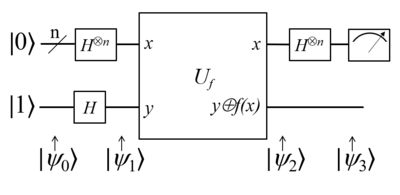
\includegraphics{400px-Deutsch-Jozsa-algorithm-quantum-circuit.png}
\\
\subsubsection{Finding the Final state}
\begin{align*}
	|0\rangle^{\otimes n}|-\rangle \xrightarrow{H^{\otimes n} \otimes \mathbb{I}} & \frac{1}{\sqrt{2^n}} \left( \sum_{x \in \{0,1\}^n} |x\rangle \right) |-\rangle                                                                            &  & \textit{Applying $H^{\otimes n} on first register set$} \\
	\xrightarrow{U_f}                                                             & \frac{1}{\sqrt{2^n}} \left( \sum_{x \in \{0,1\}^n} (-1)^{f(x)}|x\rangle \right) |-\rangle                                                                 &  & \textit{Applying phase kickback}                        \\
	\xrightarrow{H^{\otimes n} \otimes \mathbb{I}}                                & \frac{1}{\sqrt{2^n}} \left( \sum_{x \in \{0,1\}^n} (-1)^{f(x)} \frac{1}{\sqrt{2}} \left( \sum_{z \in \{0,1\}^n} (-1)^{x\cdot z} |z\rangle \right) \right) &  & \textit{Applying $H^{\otimes n} on first register set$} \\
	|\psi \rangle=                                                                & \frac{1}{2^n} \ \underset{x,z \in \{0, 1\}^n}{\sum \sum }\left( (-1)^{f(x) + x \cdot z} \ |z\rangle \right)                                               &  & \textit{Final state}                                    \\
\end{align*}

Checking the inner product of the final state with an n-bit string of $0$s,
\begin{align*}
	\langle 00 \hdots 0 | \psi \rangle & = \frac{1}{2^n} \sum_{x \in \{0, 1\}^n} (-1)^{f(x)} &  & f(x) \in \{0, 1\}                        \\
	=                                  & 1                                                   &  & \textit{if $f(x)=0$, $f(x)$ is constant} \\
	                                   & -1                                                  &  & \textit{if $f(x)=1$, $f(x)$ is constant} \\
	                                   & 0                                                   &  & \textit{if $f(x)$ is balanced}
\end{align*}

\subsubsection{Probabilities of Final State}
Finding the probabilities of the final state using the squares of amplitudes,
\begin{align*}
	\mathds{P}(|00\hdots 0\rangle) = & (\pm 1)^2 = 1 &  & \textit{ if $f(x)$ is constant} \\
	                                 & 0^2 = 0       &  & \textit{if $f(x)$ is balanced}
\end{align*}

\subsubsection{Resolving a Promise}
If $f(x)$ is constant, then the measured final state $| \psi \rangle$ will be $|00 \hdots 0\rangle$ with probability 1.\\
If $f(x)$ is balanced, then the measured final state $| \psi \rangle$ is a state other than $|00 \hdots 0\rangle$ with probability 1.

\subsubsection{Comparison}
Compared to the classical reversible computer, which needed a worst case of $\frac{2^n}{2} + 1$ queries to $C_f$, the quantum computer needs only $1$ query to $U_f$ to resolve a promise. This is an exponential speedup. Note, however, that this exponential speedup is when we must resolve the correct promise with probability $1$. If we allow for an $\varepsilon$ uncertainty to both, the speedup offered by the quantum computer will reduce to $\mathcal{O}(\log{\frac{1}{\varepsilon}})$, as seen in Assignment 1.

%2023-02-21

\section{Quantum Search - Grover's Algorithm}

Quantum search algorithms provide quadratic speedup compared to classical algorithms. That is if
it takes classical algorithms $O(N)$ steps to run, it would take a quantum algorithm $O(\sqrt{N}$
steps to run with a high probability of success.

\subsection{Problem Statement}

Let us have a set $X$ of $N=2^n$ elements
$$X = \{x_1, x_2, ... ,x_N\}$$
and a Boolean function $f: X \rightarrow \{0, 1\}$.
$x_i$ are bitstrings of length $n$. \\
Find elements $x* \in X$ such that $f(x*) = 1$. \\

The classical algorithm to solve this would always need $O(N)$ queries to the function $f$.\\

It's complexity is $O(N) = O(2^n)$ both in the average case and the worst case classically.
However the quantum approach allows us to speed this up quadratically.
This is achieved as shown below.


\subsection{The Quantum Approach}
We have seen in previous lectures the following observation:

$$H^{\otimes n}\ket{0}^{\otimes n} = \frac{1}{\sqrt{N}}\sum_{z \in {0,1}^n}\ket{z}$$

Hence the Hadamard gate when applied to $\ket{0}^{\otimes n}$ converts it to an equal superposition of all states in the computational basis. Now from now on let
$\ket{S} =\frac{1}{\sqrt{N}}\sum_{z \in {0,1}^n}\ket{z} $. \\

We now introduce a phase kickback oracle:

$$U_f: \ket{x} \rightarrow (-1)^{f(x)}\ket{x}$$

This gate will flip the phase of $\ket{x}$ for all $x*$, else it will keep the state unchanged. Applying this to our state $\ket{S}$:

$$U_f\ket{S} = \frac{1}{\sqrt{N}}(\sum_{x \notin x*}\ket{x} - \sum\ket{x*})$$

So only phase of $\ket{x*}$ is flipped. \\

\subsection{The algorithm}
The grover's algorithm is then defined as follows: \\

{
\centering
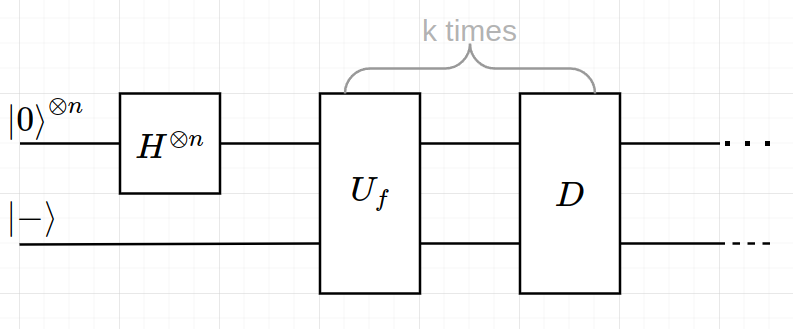
\includegraphics[width=12 cm]{algorithm.png}\par
}

$$G = (DU_f)^k\ket{S}$$

for a suitable $k$. $D$ is a gate that is called the diffuser. We now rewrite $\ket{S}$ as follows:

$$\ket{S} = \frac{1}{\sqrt{N}}\sum_{x \in \{0,1\}^n}\ket{x}$$
$$=\frac{1}{\sqrt{N}}(\sum_{x': f(x')=1}\ket{x'} + \sum_{x'': f(x'')=1}\ket{x'})$$

Now let, $|\{x: f(x) = 1\}| = M$. Define the following:

$$\ket{\omega} = \frac{1}{\sqrt{M}}\sum_{x': f(x')=1}\ket{x'}$$
$$\ket{S\omega} = \frac{1}{\sqrt{N-M}}\sum_{x'': f(x'')=0}\ket{x''}$$

Then,
$$\ket{S} = \frac{\sqrt{M}}{\sqrt{N}}\ket{\omega} + \frac{\sqrt{N-M}}{\sqrt{N}}\ket{S\omega}$$

Now we see that, $\braket{S\omega|\omega} = 0$, so the basis $\{\ket{\omega}, \ket{S\omega}\}$
forms an orthonormal set.

Let $sin(\theta/2) = \sqrt{\frac{M}{N}}$ and $cos(\theta/2) = \sqrt{\frac{N-M}{N}}$.\\          So,

$$\ket{S} = sin(\theta/2)\ket{\omega} + cos(\theta/2)\ket{S\omega}$$
$$U_f\ket{S} = -sin(\theta/2)\ket{\omega} + cos(\theta/2)\ket{S\omega}$$

\subsection{D Gate}
In the algorithm, the D gate is given by the following circuit:

{
\centering
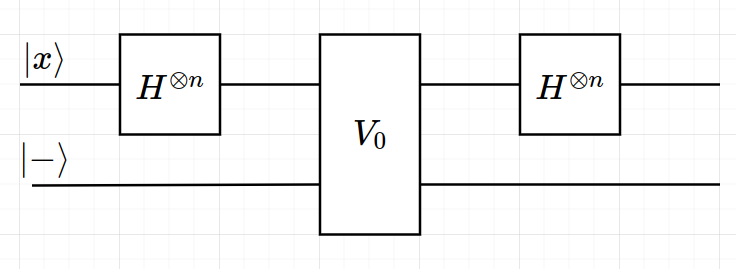
\includegraphics[width = 8 cm]{D.png}\par
}
The $V_0$ gate performs a controlled phase shift. If $\ket{x} = \ket{0}^{\otimes n}$ then
no phase shift happens, else the phase is flipped.

This gives:

$$V_0 = 2\ket{0}^{\otimes n}\bra{0}^{\otimes n} - \mathbb{I}$$

we can also write,

$$V_0 : \ket{x} \rightarrow (-1)^{OR(x_1, x_2, ...)}\ket{x}$$

since if at least one bit is non 0, there is a phase kickback.
So,

$$D = H^{\otimes n}V_0H^{\otimes n}$$
$$ = 2H^{\otimes n}\ket{0}^{\otimes n}\bra{0}^{\otimes n}H^{\otimes n} - H^{\otimes n}\mathbb{I}H^{\otimes n}$$
$$ = 2\ket{S}\bra{S} - (H^2)^{\otimes n}$$
$$ = 2\ket{S}\bra{S} - \mathbb{I}$$

\subsection{Working of the algorithm}

{
	\centering
	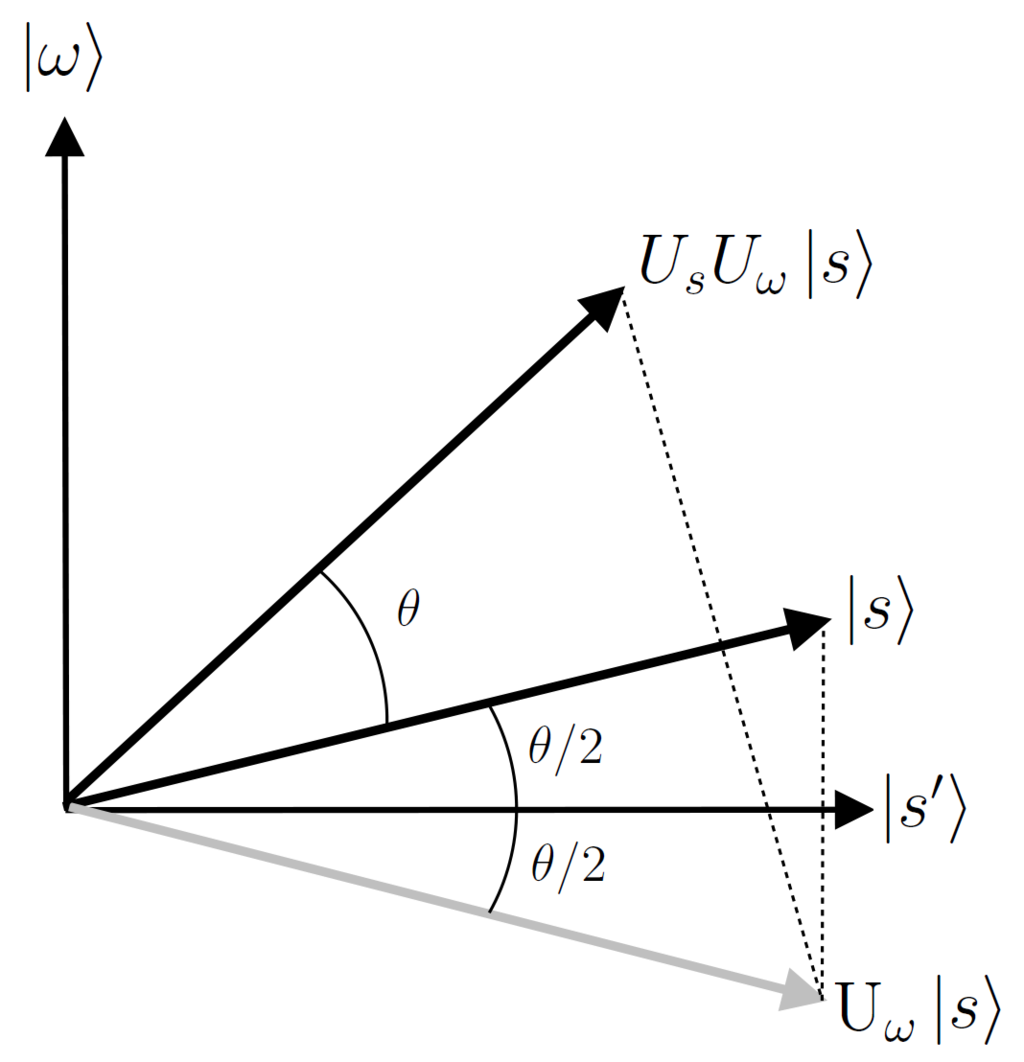
\includegraphics[width = 8 cm]{image.png}\par
}

In the above diagram of the algorithm, the $U_f$ gate flips the state along the axis for
$\ket{S\omega}$ and the $D$ gate flips it across the state $\ket{S}$. The combined effect is
a rotation by angle of $\theta$ counter clockwise on the diagram. Hence the state's overlap
with the solution state $\omega$ increases. \\

However then for the algorithm to work we must have $M << N$. This would mean $\theta$ is
considerably smaller than $\pi/2$. Then to get maximum overlap, we take $k$ as follows:

$$\theta/2 + k\theta \approx \pi/2$$

%2023-02-24

% \section{Introduction}

So S is basically 
\begin{align*}
    sin(\theta/2)]\ket{w} + cos(\theta/2)\ket{S_{\overline{w}}}
\end{align*}

$D=2\ket{S}\bra{S}-I$
\raggedright
\begin{align*}
% \raggedright
D &= 2[ \ket{w}\bra{w}sin^2(\theta/2) + \ket{w}\bra{S_{\overline{w}}}sin(\theta/2)cos(\theta/2) \\&+ \ket{S_{\overline{w}}}\bra{w}sin(\theta/2)cos(\theta/2)+ \ket{S_{\overline{w}}}\bra{S_{\overline{w}}}cos^2(\theta/2) ] - I
% \raggedright
\end{align*}

After all D is a $2\times2$ matrix \\
So in the basis {$\ket{S_{\overline{w}}},\ket{w}$} D can be represented as : 
\newline \newline
\(D = 
\begin{bmatrix}
cos(\theta) & sin(\theta) \\
sin(\theta) & -cos(\theta)
\end{bmatrix}\)
\newline
We are given $G = D\cdot u_f$
\newline\newline
\(G = 
\begin{bmatrix}
cos(\theta) & sin(\theta) \\
sin(\theta) & -cos(\theta)
\end{bmatrix}
\times
\begin{bmatrix}
1 & 0\\
0 & -1
\end{bmatrix}
\newline \newline
G = 
\begin{bmatrix}
cos(\theta) & -sin(\theta) \\
sin(\theta) & cos(\theta)
\end{bmatrix}\)

As we can see G is a rotation matrix. \\
$\ket{S} = G^k\cdot\ket{S}$\\
Let's see the product one time : 

\(  
G\ket{S} = 
\begin{bmatrix}
cos(\theta) & -sin(\theta) \\
sin(\theta) & cos(\theta)
\end{bmatrix}\ket{S}
\)\\
$G\ket{S}$ = $sin(\theta+\theta/2)\ket{w} + cos(\theta+\theta/2)\ket{S_{\overline{w}}}$\\
After k times : \\
$\ket{S}$ = $sin(k\theta+\theta/2)\ket{w} + cos(k\theta+\theta/2)\ket{S_{\overline{w}}}$\\
At that time : 
$sin(k\theta+\theta/2) = 1$\\
$\implies \theta(k+1/2)=\pi/2$\\
$\implies \theta = \frac{\pi}{2k+1}$
We know that \\
$sin(\theta/2) = \sqrt{\frac{M}{N}} \approx \theta/2$\\
$2k+1=\frac{\pi\sqrt{N}}{2\sqrt{M}}$\\
$k=\frac{\pi\sqrt{N}}{2\sqrt{M}} - \frac{1}{2}$\\
$k\approx O(\sqrt{\frac{N}{M}})$\\
So finally \\
$G^k\ket{S} = \frac{1}{\sqrt{M}} \sum_{f(\ket{x}=1)}\ket{x}$
\newline \newline
Now what if M is unknown :- \\
(a) Estimate 'M' before only  (Quantum Counting )\\
(b) Randomized Quantum Search 
\newline \newline
Amplification of amplitude : \\
$G^kH^{\otimes n}\ket{0^n} = G^k[sin(\theta/2)]\ket{w} + cos(\theta/2)\ket{S_{\overline{w}}}]$\\
$\sqrt{p}=sin(\theta/2)$\\
To amplify this term to 1 I need $\frac{1}{\sqrt{p}}$ queries.\\
$A^{\frac{1}{\sqrt{p}}}u\ket{0} \approx \ket{\psi_{good}}$

\section{Models of Quantum Computing }
1. Adiabatic Model : \\
$H(s) = (1-s)H_0+sH_k$\\
$s \in [0,1]$

2. Quantum walks \\
3. MDQC\\
4. Topological Quantum Channel \\


\end{document}
